\documentclass[Royal,times,sageh]{sagej}

\usepackage{moreverb,url,natbib, multirow, tabularx}
\usepackage[colorlinks,bookmarksopen,bookmarksnumbered,citecolor=red,urlcolor=red]{hyperref}



% tightlist command for lists without linebreak
\providecommand{\tightlist}{%
  \setlength{\itemsep}{0pt}\setlength{\parskip}{0pt}}



\usepackage{booktabs}
\usepackage{longtable}
\usepackage{array}
\usepackage{multirow}
\usepackage{wrapfig}
\usepackage{float}
\usepackage{colortbl}
\usepackage{pdflscape}
\usepackage{tabu}
\usepackage{threeparttable}
\usepackage{threeparttablex}
\usepackage[normalem]{ulem}
\usepackage{makecell}
\usepackage{xcolor}


\begin{document}


\setcitestyle{aysep={,}}

\title{Using machine learning to identify spatial market segments. A
reproducible study of major Spanish markets}

\runninghead{authors \emph{et al}.}

\author{D. Rey-Blanco\affilnum{1}, P. Arbues\affilnum{1}, F.
López\affilnum{2}, A. Páez*\affilnum{3}}

\affiliation{\affilnum{1}{Idealista, Plaza de las Cortes 5, 28014
Madrid, Spain}\\\affilnum{2}{Facultad de CC de la Empresa, C/ Real, 3.
30201 Cartagena, Murcia, Spain}\\\affilnum{3}{School of Earth,
Environment and Society, McMaster University, 1280 Main St W, Hamilton,
Ontario L8S 4K1 Canada}}

\corrauth{Antonio Páez, School of Earth, Environment and Society,
McMaster University, 1280 Main St W, Hamilton, Ontario L8S 4K1 Canada.}

\email{\href{mailto:paezha@mcmaster.ca}{\nolinkurl{paezha@mcmaster.ca}}}

\begin{abstract}
Identifying market segments can improve the fit and performance of
hedonic price models. In this paper, we present a novel approach to
market segmentation based on the use of machine learning techniques.
Concretely, we propose a two-stage process. In the first stage,
classification trees with interactive basis functions are used to
identify non-orthogonal and non-linear sub-market boundaries. The market
segments that result are then introduced in a spatial econometric model
to obtain hedonic estimates of the implicit prices of interest. The
proposed approach is illustrated with a reproducible example of three
major Spanish real estate markets. We conclude that identifying market
subsegments using the approach proposed is a relatively simple and
demonstrate the potential of the proposed modelling strategy to produce
better models and more accurate predictions.
\end{abstract}

\keywords{Hedonic prices; market segments; decision trees; spatial
econometrics; reproducible research;}

\maketitle

\newpage

\hypertarget{introduction}{%
\section{Introduction}\label{introduction}}

Hedonic price analysis is one of the most widely-used approaches for the
study and valuation of properties in real estate markets. This approach
is attractive due to its strong theoretical grounding and appealing
interpretation \citep{Rosen1974hedonic}. Indeed, when hedonic price
models are estimated using multiple linear regression the coefficients
of the model are thought to capture the implicit prices of attributes in
a bundled good. In this way, while a room may lack an explicit price in
the valuation of a property, the coefficient of a hedonic price model
quantifies its implicit value. Such decomposition of the price of a
bundled good into the implicit prices of its constituent parts is
important for multiple reasons: this analysis is the industry standard
for property assessment for tax purposes \citep{Morillo2017application};
these models are used to quantify the willingness to pay for non-market
environmental amenities \citep{Montero2018estimating}, including air
quality and open spaces and similarly they can be used to assess the
cost of disamenities \citep[e.g.,][]{vonGraevenitz2018amenity}.

The need to assess property values in a transparent, accurate, and
precise way has led to numerous developments. A strand of research has
aimed at enhancing the performance of models by incorporating spatial
information. Geographic Information Systems (GIS) in particular have
been used to make explicit some attributes of properties and their
environments that might otherwise be overlooked \citep{Paterson2002out}.
The use of spatial data, in turn, has brought increased attention to the
question of statistical sufficiency and therefore the need for
approaches that appropriately consider the issues of spatial association
and spatial heterogeneity in hedonic price analysis
\citep{Pace1997spatial, Paez2001spatial}. As a result, there has been a
proliferation of studies that apply spatial statistical or econometric
methods to the issue of property valuation \citep{Paez2009recent}.
Recent applications include the use of hierarchical spatial
autoregressive models \citep{Cellmer2019application}, moving windows
approaches \citep{Paez2008moving}, spatial filtering
\citep{Helbich2016spatially}, and kriging techniques
\citep{Montero2009estimating}, among others.

In addition to interest in spatial data, the application of machine
learning techniques for hedonic price analysis has also become an active
topic of research. There are at least two distinct ways in which machine
learning can be used for hedonic price analysis. In some studies, the
role of machine learning algorithms is to process information that would
otherwise be difficult or impossible to obtain using non-automated
means. The information obtained is then used as an input in econometric
hedonic models. For example, \citet{Humphreys2019superstition} and
\citet{Nowak2018homeowner} used machine learning classifiers to
ethnically profile buyers and sellers based on last names to understand
whether potential cultural biases and/or discrimination issues exist in
property transactions. In other research, machine learning algorithms
replace the conventional hedonic price model
\citep{Hu2019monitoring, Yoo2012variable, Fuss2016role}. The evidence
available shows that machine learning methods can perform remarkably
well, but can also be seen as black boxes\footnote{An emergent body of
  research aims at increasing the interpretability of machine learning
  methods, including \citet{du2019techniques} and
  \citet{murdoch2019definitions}, among others. This is an area of
  research that is quickly evolving, although it is not without critics
  \citep[e.g.,][]{rudin2019stop}. Currently, existing approaches depend
  on fairly strong assumptions. For example, the causal forest framework
  \citep{wager2018estimation, knaus2021machine} assumes that the leaves
  of trees are sufficiently small to mimic a randomized experiment.
  Assuming independence is often inappropriate in the analysis of
  spatial data, and econometric techniques that correctly treat spatial
  dependencies are mature. It is possible that in the future
  interpretable machine learning techniques will address spatial
  dependencies as well, so we are advised to pay attention to this
  stream of research.} with low interpretability \citep[see page 25
in][]{James2013introduction}.

Our objective in this paper is to introduce a novel approach that
retains the interpretability of econometric approaches, but is enhanced
by the identification of spatial market segments obtained from the use
of machine learning techniques. We propose a two-stage approach. In the
first stage, classification trees are implemented to identify
homogeneous spatial market segments. The number of market segments is
endogenous, and, compared to \citet{Fuss2016role}, the use of
interactive basis functions \citep[see][]{Paez2019inducing} can
accommodate non-orthogonal and non-linear decision boundaries. The
market segments are then introduced as covariates in an econometric
model. This approach can potentially enhance the model without
compromising its interpretability.

A reproducible case study of property values in three major markets in
Spain helps to illustrate the proposed approach. Following
recommendations for openness and reproducibility in geospatial research
\citep{Paez2021open}, this paper is accompanied by a fully documented
and open data product \citep[see][]{arribas2021open}, and the code is
embedded in a self-contained Rmarkdown document. The results show that
modeling prices using the approach proposed to identify spatial market
segments improves the fit of the models and can in addition enhance the
quality of predictions.

\hypertarget{spatial-market-segmentation}{%
\section{Spatial Market
Segmentation}\label{spatial-market-segmentation}}

The importance of housing submarkets has long been recognized in the
literature \citep[e.g.][]{Rapkin1953housing}. Market differentiation can
be the result of a variety of processes operating separately or in
conjunction, including substitution, differentiation, and variations in
consumer preferences \citep{Galster1996william}. In principle, this
implies a degree of homogeneity within the market segment that
differentiates it from other segments. According to Thibodeau
\citeyearpar[pp.~4-5]{Thibodeau2003marking} a spatial housing submarket
``defines a geographic area where the price of housing per unit of
housing service is constant''. Given the non-tradeable nature of
location, research has shown the relevance of spatial market segments
\citep{Bourassa2007spatial, Royuela2013heuristic, Usman2020property}.

Submarket analysis is often implemented in a pragmatic way, encompassing
regional boundaries, for instance those of metropolitan regions, cities,
or municipalities. It has long been recognized, though, that sub-markets
may exist at smaller scales \citep[e.g.,][]{Rapkin1953housing}. In
particular, the pioneering work of Alonso \citep{Alonso1964location} on
urban structure led to the realization of the importance of geography in
terms of differentiation of real estate property. Since then, vast
amounts of empirical evidence have contributed to demonstrate just how
commonplace differences in hedonic prices are at the intraurban scale.
Concurrently, market segmentation has been shown to be not only a
conceptually sound practice \citep[see][]{Watkins2001definition}, but
also conducive to higher quality models and improved predictive
performance, in particular when geography is explicitly taken into
consideration \citep{Paez2008moving}.

Numerous approaches have been proposed to identify market segments. Some
are based on expert opinion, such as from appraisers
\citep{Wheeler2014bayesian}. Many others are data-driven, using
statistical or machine learning techniques
\citep[e.g.,][]{Helbich2013data, Wu2018modified}. Heuristic approaches
also exist that exploit the latent homogeneity in values
\citep{Royuela2013heuristic}. Implementation of market segments in
hedonic price models can be accomplished by means of fixed effects
(i.e., dummy variables) for sub-regions
\citep[e.g.,][]{Bourassa2007spatial}, spatial drift by means of a trend
surface \citep[e.g.][]{Pace1997spatial}, spatially autoregressive models
\citep[e.g.,][]{Pace1998spatiotemporal}, switching regressions
\citep[e.g.,][]{Islam2011addressing, Paez2001spatial}, multilevel and/or
Bayesian models \citep[e.g.,][]{Wheeler2014bayesian}, or by means of
spatially moving windows or non-parametric techniques to obtain soft
market segments \citep{Paez2008moving, Hwang2009delineating}. As is
commonly the case, there is no one technique that performs consistently
better than the alternatives in every case, since performance depends to
some extent on the characteristics of the process being modeled
\citep{Usman2020property}. It is therefore valuable to explore
alternative approaches to identify and model market segments, to further
enrich the repertoire of techniques available to analysts.

A recent proposal along these lines is due to \citet{Fuss2016role}, who
suggest using decision trees to identify and model market segments.
\citet{James2013introduction} list some attractive features of decision
trees. They are relatively simple to estimate and intuitive to
interpret. They divide attribute space into a set of mutually exclusive
and collectively exhaustive regions, and thus are ideally suited for
market segmentation. By design, the regions generated are spatially
compact and internally homogeneous. And they can outperform other
regression techniques. Market segments derived from a decision tree can
be used in combination with other modeling techniques, such as a
second-stage tree regression (with fixed effects for the market segments
from the preliminary tree regression), linear models, or models with
spatial or spatio-temporal effects, such as space-time autoregression.
\citet{Fuss2016role} compare several different modeling techniques.
Their findings confirm that introducing a form of market segmentation
greatly improves prediction accuracy, and the use of tree-based market
segments does so more than the use of an \emph{a priori} zoning system
defined by ZIP codes. Furthermore, accounting for residual spatial
pattern in the form of a spatial autoregressive model further improves
the accuracy of estimation.

The results reported by \citet{Fuss2016role} are appealing. However, the
modeling strategy that they implement inherits a limitation of tree
regression, namely the relatively inflexible way in which attribute
space is partitioned using recursive binary splits. What this means is
that market segments obtained in this way are limited to linear and
orthogonal boundaries \citep[see page 1359 in][]{Fuss2016role}. While
prediction accuracy reportedly improves with tree-based segmentation of
the market, it might be desirable to define market segments more
flexibly, so that they are not constrained to rectangular shapes.
Secondly, estimates of a regression tree are the mean of the values
contained in the volume of a leaf, which means they are constants for
each leaf. In a geographical application the leaves are mutually
exclusive and collectively exhaustive partitions of geographical space.
Using the residuals in the second step of the modelling strategy induces
spatial autocorrelation, since all properties in the same segment will
be given estimated residuals that are constants in each market segment.
The issue here is that by introducing spatial autocorrelation in the
second step some of the spatial information about location is obscured
since there is zero spatial variation in the estimated residuals for a
given market segment.

We address these two issues by using interactive basis functions
\citep{Paez2019inducing} to induce non-orthogonal and non-linear
decision boundaries in our models of market segments. Further, by moving
the analysis of market segments to the first stage of the analysis, we
obtain market segments with good homogeneity properties, and any spatial
autocorrelation is dealt with by means of the spatial econometric model
in the second step. The modelling strategy is described in more detail
next.

\hypertarget{modeling-strategy-and-methods}{%
\section{Modeling Strategy and
Methods}\label{modeling-strategy-and-methods}}

\hypertarget{modeling-strategy}{%
\subsection{Modeling Strategy}\label{modeling-strategy}}

We propose a two-stage modelling strategy, as follows:

\begin{enumerate}
\def\labelenumi{\arabic{enumi}.}
\tightlist
\item
  Estimate a first stage classification tree using the prices and the
  coordinates of the observations only \citep[similar to trend surface
  analysis, see][]{Unwin1978introduction}.
\end{enumerate}

\begin{itemize}
\tightlist
\item
  Map the regions \(R_m\) that result: these are the \(m=1,\cdots,M\)
  submarkets.
\item
  Overlay the observations on the tree-based regions and create a set of
  \(m\) indicator variables for submarket membership:
  \(I_m=I(y_i\in R_m)\); when the argument of the indicator function is
  true (i.e., when observation \(y_i\) is in \(R_m\)) then \(I_m=1\),
  otherwise \(I_m=0\).
\end{itemize}

\begin{enumerate}
\def\labelenumi{\arabic{enumi}.}
\setcounter{enumi}{1}
\tightlist
\item
  Estimate a second-stage hedonic price model that incorporates the
  indicator variables for submarkets obtained in first stage including
  spatial interaction effects and other relevant covariates.
\end{enumerate}

Note that the modeling strategy proposed here differs from the one
proposed by \citet{Fuss2016role} in that the market areas are identified
by these authors based on the residuals of a preliminary regression,
whereas we identify them based on the prices directly. It is worth
noting that these two strategies reflect different heuristics.
Identification of market areas based on the prices implies that market
areas are formed based on unitary properties before properties are
assessed as bundles of attributes. Identification of market areas based
on the residuals, on the other hand, implies that properties are first
seen as bundles of attributes and that submarkets form based on other
non-identified attributes.

\hypertarget{methods}{%
\subsection{Methods}\label{methods}}

Two methodologies are combined in the modeling strategy. For first-stage
we apply the well-known algorithm of classification trees with the
objective of identify spatial submarkets. The algorithm is applied using
the variation suggested by \citet{Paez2019inducing} to obtain
non-orthogonal and non-linear boundaries via interactive basis
functions. A short description of this method is found in the
supplementary material. For the second-stage we apply spatial
econometric methods to solve the presence of spatial autocorrelation in
the residual of the classical hedonic models. The patial econometric
models considered are also briefly described in the supplementary
material. These methods are implemented in a number of open-source R
packages. The \textbf{tree} R package \citep{tree} was used in
first-stage and \textbf{spsur} \citep{lopez2020} and \textbf{spatialreg}
\citep{bivand2013} in second-stage to estimate spatial regression
models. Finally, with the objective of evaluate the forecasting
accuracies of the different models and avoid overfitting the data set is
split in training and test subsamples. The training subsample is used to
obtain the model and the test subsample to evaluate the forecasting. The
R package \textbf{spatialreg} is used to get the out-of-sample
predictions is a spatial econometric framework.

\hypertarget{data}{%
\section{Data}\label{data}}

The empirical examples to follow correspond to large cities in Spain.
The real estate market is one of the most important sectors of the
Spanish economy, and the largest urban areas in Spain are important
points of reference for the real estate market in the country. The three
largest markets are Madrid (the national capital with 3.2 million
inhabitants), Barcelona (1.6 million), and Valencia (0.8 million
inhabitants). The focus of our application is on property prices in
these cities. Micro-data from official sources are not available in
Spain; instead, we draw our data from an online real estate database,
Idealista.com (the leading real estate portal in Spain).

The data are documented and prepared for sharing publicly in the form of
an open data product \citep{arribas2021open} under the structure of a R
package free available from a
repository\footnote{\url{https://paezha.github.io/idealista18/}} and a
data paper describe the full data set. The database is for postings
during 2018, and the analysis uses the last quarter of the year. We use
the asking price as a proxy for the selling price; this is common
practice in many real estate studies
\citep[e.g.,][]{lopez2015, chasco2018}. For the three data sets we
consider the most frequent type of property in Spain, namely the flat
(hereon termed ``houses''); this excludes other types of properties,
such as duplex, chalets, and attics, which conform separate real estate
markets.

The data sets used in the analysis correspond to the last quarter of
2018, and include a total of \(n=\) 44,270 for Madrid, \(n=\) 23,334 for
Barcelona, and \(n=\) 14,018 for Valencia. The distribution of prices
displays a long tail in all three cities, and following conventional
practice it is log-transformed. The coordinates are converted from
latitude and longitude to northing and easting in meters, and then
rescaled and centered using the corresponding city's Central Business
District as a false origin. These transformations have no impact on the
analysis, and rescaling and centering of the coordinates is necessary
for the correct implementation of the interactive basis functions in
decision trees \citep[see][pp.~188-189]{Paez2019inducing}.

For this research we select thirteen explanatory variables. Of these,
ten attributes are data provided by Idealista.com and represent key
structural attributes of the properties. These are whether the property
is a studio (a small type of bachelor apartment), whether it is on the
top floor of the building, and its built area, number of rooms, number
of baths, and presence of a terrace. In addition, there are variables
for elevator in the building, air conditioner, swimming pool, and
parking spaces. We augment these attributes with locational variables
derived from the coordinates of the property, including distance to
nearest major transit station (metro), distance to the city center
(central business district; CBD), and distance to major avenues. These
locational attributes are frequently advertised by real estate agents
and often capitalized in housing prices. Table \ref{tab:descriptives}
gives the definitions of these variables and the descriptive statistics
of the data.

\begin{table}[ht]
\centering
\fontsize{6}{8}\selectfont
\begin{tabular}{>{\raggedright\arraybackslash}p{12em}>{\raggedright\arraybackslash}p{16em}cccccc}
  \toprule
\multicolumn{2}{c}{ } & \multicolumn{2}{c}{ Barcelona} & \multicolumn{2}{c}{Madrid} & \multicolumn{2}{c}{Valencia} \\
\cmidrule(l{3pt}r{3pt}){3-4} \cmidrule(l{3pt}r{3pt}){5-6} \cmidrule(l{3pt}r{3pt}){7-8}
Variable & Description & mean & std & mean & std & mean & std \\ 
  \midrule
CONSTRUCTEDAREA & Home built area in sq.m & 95.46 & 52.58 & 101.40 & 67.08 & 108.95 & 47.29 \\ 
  ROOMNUMBER & Number of bedrooms & 2.86 & 1.13 & 2.58 & 1.24 & 3.07 & 1.09 \\ 
  BATHNUMBER & Number of bathrooms & 1.52 & 0.71 & 1.59 & 0.84 & 1.59 & 0.64 \\ 
  HASTERRACE & =1 if has terrace, 0 otherwise & 0.33 & 0.47 & 0.36 & 0.48 & 0.25 & 0.44 \\ 
  HASLIFT & =1 if has lift, 0 otherwise & 0.74 & 0.44 & 0.70 & 0.46 & 0.79 & 0.41 \\ 
  HASAIRCONDITIONING & =1 if has air conditioner, 0 otherwise & 0.47 & 0.50 & 0.45 & 0.50 & 0.47 & 0.50 \\ 
  HASSWIMMINGPOOL & =1 if has swimming pool, 0 otherwise & 0.03 & 0.16 & 0.15 & 0.36 & 0.07 & 0.26 \\ 
  ISSTUDIO & =1 if is studio apartment, 0 otherwise & 0.02 & 0.13 & 0.03 & 0.16 & 0.01 & 0.08 \\ 
  ISINTOPFLOOR & =1 is on the top floor, 0 otherwise & 0.02 & 0.14 & 0.02 & 0.15 & 0.01 & 0.12 \\ 
  HASPARKINGSPACE & =1 if has parking, 0 otherwise & 0.08 & 0.27 & 0.23 & 0.42 & 0.17 & 0.37 \\ 
  DISTANCE\_TO\_CITY\_CENTER & Distance to nearest subway station (km) & 2.80 & 1.56 & 4.49 & 2.99 & 2.09 & 0.97 \\ 
  DISTANCE\_TO\_METRO & Distance to city center (km) & 0.27 & 0.16 & 0.48 & 1.43 & 0.64 & 0.42 \\ 
  DISTANCE\_TO\_(Avenue) & Distance to major avenue (km) & 1.77 & 1.15 & 2.68 & 2.58 & 2.07 & 1.09 \\ 
   \bottomrule
\end{tabular}
\caption{Sort description and descriptive statistics (Fourth Quarter of 2018)\label{tab:descriptives}} 
\end{table}

\hypertarget{empirical-examples}{%
\section{Empirical Examples}\label{empirical-examples}}

\hypertarget{experimental-design}{%
\subsection{Experimental Design}\label{experimental-design}}

Each city's data set is split into a training sample and a testing
sample using a 7:3 proportion. The training samples are used to estimate
the models and the testing samples are used to assess the out-of-sample
performance of the models.

We consider four models. First is a Base Model:

\begin{equation}
y_i = \ \sum_{j=1}^{k}{\beta_{j} x_{ij}} + \epsilon_i \ \ (i=1,...,n)
\label{eq:base-model}
\end{equation}

The second is a base model with market segments (Base Model + MS):

\begin{equation}
y_i = \sum_{m=2}^{M}{\gamma_{m} I(y_i\in R_m)} + \ \sum_{j=1}^{k}{\beta_{j} x_{ij}} + \epsilon_i \ \ (i=1,...,n)
\label{eq:base-model-ms}
\end{equation}

The third is a spatial lag model (Spatial Model):

\begin{equation}
y_i = \rho {1 \over n_i } \sum_{j=1}^{n_i}{Y_j} \ + \ \sum_{j=1}^{k}{\beta_{j} x_{ij}} + \epsilon_i \ \ (i=1,...,n)
\label{eq:spatial-model}
\end{equation}

And finally, the most general is a spatial lag model with market
segments (Spatial Model + MS):

\begin{equation}
y_i = \rho {1 \over n_i } \sum_{j=1}^{n_i}{Y_j} \ + \ \sum_{m=2}^{M}{\gamma_{m} I(y_i\in R_m)} + \ \sum_{j=1}^{k}{\beta_{j} x_{ij}} + \epsilon_i \ \ (i=1,...,n)
\label{eq:spatial-model-ms}
\end{equation}

Please note that all models nest in the Spatial Model + MS depending on
what restrictions are placed on the parameters. In the Base Model:

\begin{equation}
\rho = \gamma_{m} = 0\ \ (\forall m)
\label{eq:restrictions-base}
\end{equation}

In the Base Model + MS:

\begin{equation}
\rho = \ 0\ 
\label{eq:restrictions-base}
\end{equation}

And in the Spatial Model:

\begin{equation}
\gamma_{m} = 0\ \ (\forall m)
\label{eq:restrictions-base}
\end{equation}

The weights in the spatial weight matrices are calculated using the
inverse of the distance between neighboring observations, so that closer
observations receive a higher weight. To avoid increasing the density of
the matrices {[}which has computational and also estimation effects{]},
we combine this criterion with a cutoff of \(k=6\) nearest neighbors.
Given the distribution of distances in the sample, beyond these
neighbors the inverse distance results in extremely small contributions
to the autocorrelation effect. With respect to the interactive basis
functions for the decision trees, we consider the following functions
(see supplementary material) with \(u\) and \(v\) as the planar
coordinates of the observations, easting and northing respectively:

\begin{equation}
\begin{array}{ccc}
u_i + v_i \\ [5pt]
u_i^2 + v_i^2 \\ [5pt]
u_i \cdot v_i
\end{array}
\label{eq:ibf1}
\end{equation}

We first look at the estimated models before discussing the in- and
out-of-sample predictive performance of the models.

\hypertarget{modelling-results}{%
\subsection{Modelling Results}\label{modelling-results}}

The first model in each of Tables \ref{tab:model-results-barcelona},
\ref{tab:model-results-madrid}, and \ref{tab:model-results-valencia} is
the Base Model. The fit of these models is reasonably high: the adjusted
coefficients of determination are \(R^2=\) 0.796, \(R^2=\) 0.777, and
\(R^2=\) 0.795 for Barcelona, Madrid, and Valencia, respectively. These
models are relatively naive in that they disregard both the possibility
of spatial autocorrelation and spatial heterogeneity (in the form of
spatial market sub-segments). They do provide a useful benchmark to
compare the proposed modelling strategy.

The first stage of the modelling strategy is to train a decision tree on
the property values using only the coordinates of the observations. The
spatial market sub-segments derived from the decision trees are shown in
Figure \ref{fig:all-market-segments}. It can be seen there that the
algorithm detects seven market sub-segments in Barcelona, nine market
sub-segments in Madrid, and eight in Valencia. These submarkets are
compact, mutually exclusive, and collectively exhaustive. The smallest
market segment is found in Valencia and has 331 recorded transactions;
the largest market segment, in contrast, has 7,816 recorded transactions
and is found in Madrid. The maps in the figure show how the use of
interactive basis functions leads to non-orthogonal/non-linear
boundaries for the sub-markets. In the case of Barcelona, there are some
distinctive diagonal shapes reminiscent of the street pattern in the
city. In Madrid there is a clear distinction given by the M-30 orbital
that surrounds the central almond of the city; in addition, there is
Paseo de la Castellana, a major north-south avenue that crosses the
city. This avenue divides two zones in the north that tend to include
more expensive real estate, whereas the south tends to be lower income
and less expensive. In Valencia, the sub-markets identify several zones
in the historical center of the city, and then larger regional patterns
depending on proximity to the waterfront to the west of the city.

\begin{figure}
\centering
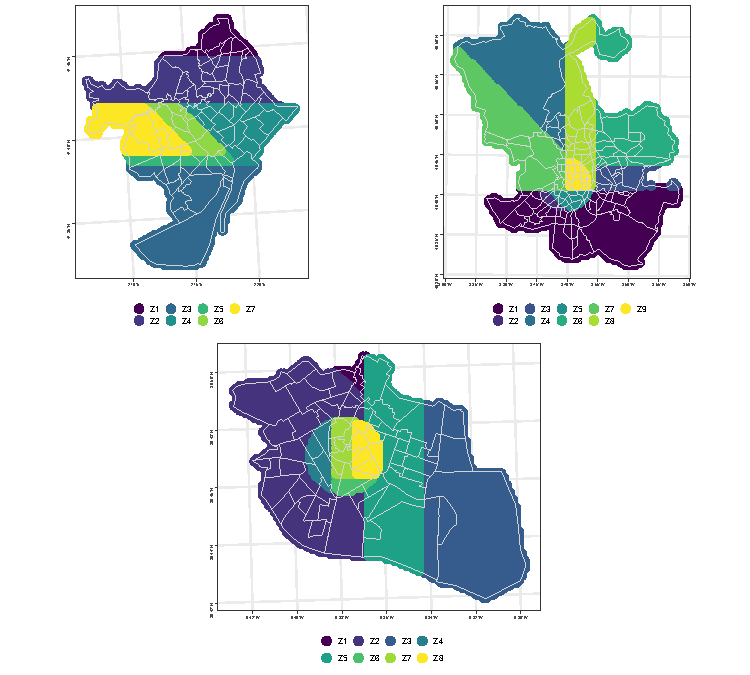
\includegraphics{EPB-preprint_files/figure-latex/unnamed-chunk-1-1.pdf}
\caption{\label{fig:all-market-segments}Spatial market segments
according to Stage 1 classification tree. Barcelona (upper-left), Madrid
(upper-right), and Valencia (botton-center)}
\end{figure}

The spatial market sub-segments are coded as dummy variables in the data
sets before re-estimating the Base Model with market segments (Base
Model + MS). The second model reported in Tables
\ref{tab:model-results-barcelona}, \ref{tab:model-results-madrid}, and
\ref{tab:model-results-valencia} shows that the market segments tend to
be highly significant, and also improve the fit of the model. In the
case of Barcelona, the adjusted coefficient of determination changes to
\(R^2=\) 0.821, for a modest increase of 3.19\%. The introduction of the
market segments into the Base Model for Madrid results in an adjusted
coefficient of determination of \(R^2=\) 0.878, which represents a
change of 13.09\% relative to the adjusted coefficient of determination
of the Base Model. In Valencia, the Base Model with market segments has
an adjusted coefficient of determination of \(R^2=\) 0.83, for an
increase with respect to the Base Model of 4.49\%.

It is well-known that spatial heterogeneity and association can co-exist
\citep[e.g.,][]{Bourassa2007spatial, Paez2001spatial}. Sub-market
identification can assist with spatial heterogeneity, but a process of
spatial association could result from the common heuristic of
comparative sales used by real estate agents. This process is
appropriately represented by a spatial lag model. The third model
reported in Tables \ref{tab:model-results-barcelona},
\ref{tab:model-results-madrid}, and \ref{tab:model-results-valencia} is
the Spatial Model, that is the Base Model with a spatial lag (i.e.,
Equation \ref{eq:spatial-model}). Spatial lag models, being non-linear,
lack the coefficient of determination of linear regression. Instead,
their goodness of fit is evaluated using likelihood measures. It can be
seen that there is a substantial improvement in this regard in all three
cities. The spatial lag parameter \(\rho\) represents the proportion of
the mean of the neighboring prices that is reflected in the price of the
property at \(i\). In Barcelona, this parameter suggests that
approximately 32.16\% of the mean of the price of the \(k=6\) nearest
neighbors is reflected in the price at \(i\). This ``comparative sales''
effect is markedly stronger in Madrid, where it amounts to 47.89\% of
the mean price of the neighbors. In Valencia, this effect is 40.31\%.
The spatial lag parameter is significant in all three cases, and the
results suggest that comparisons with other properties play a larger
role in the determination of prices in Madrid.

The last model that we consider for these case studies is a spatial lag
model with market segments. This is the most general of the four models,
and we see that the combination of market segments and a spatial lag
variable gives the best fit in terms of the log-likelihood, and also
reduces the size of the spatial lag coefficient, shifting some of the
spatial effect from spatial autocorrelation to spatial heterogeneity.

At this point, it is important to note that the coefficients of models
with spatial lags cannot be interpreted as marginal effects due to the
ripple effects of lagging variables (i.e., the multiplier effect of the
lag). Instead, the direct, indirect, and total impacts need to be
considered. The impacts of our best models (spatial models with market
segments) are presented in Tables \ref{tab:model-impacts-barcelona},
\ref{tab:model-impacts-madrid}, and \ref{tab:model-impacts-valencia}.

\begin{table}

\caption{\label{tab:table-models-barcelona}\label{tab:model-results-barcelona}Models Barcelona (Dependent Variable is log of Price)}
\centering
\resizebox{\linewidth}{!}{
\begin{tabular}[t]{lcccccccc}
\toprule
\multicolumn{1}{c}{ } & \multicolumn{2}{c}{Base Model} & \multicolumn{2}{c}{Base Model + MS} & \multicolumn{2}{c}{Spatial Model} & \multicolumn{2}{c}{Spatial Model + MS} \\
\cmidrule(l{3pt}r{3pt}){2-3} \cmidrule(l{3pt}r{3pt}){4-5} \cmidrule(l{3pt}r{3pt}){6-7} \cmidrule(l{3pt}r{3pt}){8-9}
Variable & Estimate & p-val & Estimate & p-val & Estimate & p-val & Estimate & p-val\\
\midrule
\addlinespace[0.3em]
\multicolumn{9}{l}{\textbf{Property attributes}}\\
\hspace{1em}(Intercept) & 11.9207 & 0.001 & 11.5877 & 0.001 & 7.9308 & 0.001 & 8.4258 & 0.001\\
\hspace{1em}CONSTRUCTEDAREA & 0.0058 & 0.001 & 0.0053 & 0.001 & 0.0048 & 0.001 & 0.0048 & 0.001\\
\hspace{1em}ROOMNUMBER & 0.0233 & 0.001 & 0.0255 & 0.001 & 0.0239 & 0.001 & 0.0243 & 0.001\\
\hspace{1em}BATHNUMBER & 0.1351 & 0.001 & 0.1164 & 0.001 & 0.1026 & 0.001 & 0.1004 & 0.001\\
\hspace{1em}HASTERRACE & 0.0785 & 0.001 & 0.0799 & 0.001 & 0.074 & 0.001 & 0.0752 & 0.001\\
\hspace{1em}HASLIFT & 0.2302 & 0.001 & 0.1962 & 0.001 & 0.165 & 0.001 & 0.1583 & 0.001\\
\hspace{1em}HASAIRCONDITIONING & 0.1095 & 0.001 & 0.1093 & 0.001 & 0.1017 & 0.001 & 0.1024 & 0.001\\
\hspace{1em}HASSWIMMINGPOOL & 0.1572 & 0.001 & 0.1508 & 0.001 & 0.129 & 0.001 & 0.127 & 0.001\\
\hspace{1em}ISSTUDIO & -0.2628 & 0.001 & -0.2568 & 0.001 & -0.237 & 0.001 & -0.2386 & 0.001\\
\hspace{1em}ISINTOPFLOOR & 0.0408 & 0.0045 & 0.0476 & 0.001 & 0.0441 & 0.001 & 0.0456 & 0.001\\
\hspace{1em}HASPARKINGSPACE & 0.1385 & 0.001 & 0.0806 & 0.001 & 0.0726 & 0.001 & 0.0585 & 0.001\\
\hspace{1em}DISTANCE\_TO\_CITY\_CENTER & -0.1023 & 0.001 & -0.0611 & 0.001 & -0.0664 & 0.001 & -0.0469 & 0.001\\
\addlinespace[0.3em]
\multicolumn{9}{l}{\textbf{Market segments}}\\
\hspace{1em}market\_segmentZ2 & - & - & 0.1572 & 0.001 & - & - & 0.0885 & 0.001\\
\hspace{1em}market\_segmentZ3 & - & - & 0.2761 & 0.001 & - & - & 0.1697 & 0.001\\
\hspace{1em}market\_segmentZ4 & - & - & 0.3654 & 0.001 & - & - & 0.2191 & 0.001\\
\hspace{1em}market\_segmentZ5 & - & - & 0.4102 & 0.001 & - & - & 0.2381 & 0.001\\
\hspace{1em}market\_segmentZ6 & - & - & 0.5074 & 0.001 & - & - & 0.2739 & 0.001\\
\hspace{1em}market\_segmentZ7 & - & - & 0.5605 & 0.001 & - & - & 0.2541 & 0.001\\
\addlinespace[0.3em]
\multicolumn{9}{l}{\textbf{Spatial lag parameter}}\\
\hspace{1em}rho & - & - & - & - & 0.3216 & 0.001 & 0.2647 & 0.001\\
\addlinespace[0.3em]
\multicolumn{9}{l}{\textbf{Model diagnostics}}\\
\hspace{1em}R-squared &  & 0.8 &  & 0.82 &  & - &  & -\\
\hspace{1em}adj-R-squared: &  & 0.8 &  & 0.82 &  & - &  & -\\
\hspace{1em}log-likelihood: &  & -781.44 &  & 303.91 &  & 989.45 &  & 1247.72\\
\bottomrule
\end{tabular}}
\end{table}

\begin{table}

\caption{\label{tab:table-models-madrid}\label{tab:model-results-madrid}Models Madrid (Dependent Variable is log of Price)}
\centering
\resizebox{\linewidth}{!}{
\begin{tabular}[t]{lcccccccc}
\toprule
\multicolumn{1}{c}{ } & \multicolumn{2}{c}{Base Model} & \multicolumn{2}{c}{Base Model + MS} & \multicolumn{2}{c}{Spatial Model} & \multicolumn{2}{c}{Spatial Model + MS} \\
\cmidrule(l{3pt}r{3pt}){2-3} \cmidrule(l{3pt}r{3pt}){4-5} \cmidrule(l{3pt}r{3pt}){6-7} \cmidrule(l{3pt}r{3pt}){8-9}
Variable & Estimate & p-val & Estimate & p-val & Estimate & p-val & Estimate & p-val\\
\midrule
\addlinespace[0.3em]
\multicolumn{9}{l}{\textbf{Property attributes}}\\
\hspace{1em}(Intercept) & 11.8006 & 0.001 & 11.318 & 0.001 & 5.9368 & 0.001 & 8.1051 & 0.001\\
\hspace{1em}CONSTRUCTEDAREA & 0.0055 & 0.001 & 0.0045 & 0.001 & 0.0038 & 0.001 & 0.0039 & 0.001\\
\hspace{1em}ROOMNUMBER & -0.0068 & 0.0087 & 0.0345 & 0.001 & 0.0223 & 0.001 & 0.0368 & 0.001\\
\hspace{1em}BATHNUMBER & 0.1653 & 0.001 & 0.1163 & 0.001 & 0.0999 & 0.001 & 0.0958 & 0.001\\
\hspace{1em}HASTERRACE & -0.0098 & 0.0265 & 0.0459 & 0.001 & 0.0202 & 0.001 & 0.0436 & 0.001\\
\hspace{1em}HASLIFT & 0.3809 & 0.001 & 0.2527 & 0.001 & 0.2175 & 0.001 & 0.2022 & 0.001\\
\hspace{1em}HASAIRCONDITIONING & 0.1036 & 0.001 & 0.0878 & 0.001 & 0.0871 & 0.001 & 0.0841 & 0.001\\
\hspace{1em}HASSWIMMINGPOOL & 0.2119 & 0.001 & 0.1961 & 0.001 & 0.0895 & 0.001 & 0.129 & 0.001\\
\hspace{1em}ISSTUDIO & -0.1746 & 0.001 & -0.1827 & 0.001 & -0.1497 & 0.001 & -0.1671 & 0.001\\
\hspace{1em}ISINTOPFLOOR & 0.0256 & 0.0565 & 0.0225 & 0.0233 & 0.0361 & 0.001 & 0.0296 & 0.0012\\
\hspace{1em}HASPARKINGSPACE & 0.0885 & 0.001 & 0.1197 & 0.001 & 0.0598 & 0.001 & 0.0915 & 0.001\\
\hspace{1em}DISTANCE\_TO\_METRO & 0.033 & 0.001 & -0.0414 & 0.001 & -0.0065 & 0.001 & -0.0394 & 0.001\\
\hspace{1em}DISTANCE\_TO\_CITY\_CENTER & -0.0474 & 0.001 & -0.0484 & 0.001 & -0.0301 & 0.001 & -0.0394 & 0.001\\
\hspace{1em}DISTANCE\_TO\_CASTELLANA & -0.0631 & 0.001 & 0.0195 & 0.001 & -0.0215 & 0.001 & 0.0175 & 0.001\\
\addlinespace[0.3em]
\multicolumn{9}{l}{\textbf{Market segments}}\\
\hspace{1em}market\_segmentZ2 & - & - & 0.0663 & 0.001 & - & - & 0.047 & 0.001\\
\hspace{1em}market\_segmentZ3 & - & - & 0.2286 & 0.001 & - & - & 0.1643 & 0.001\\
\hspace{1em}market\_segmentZ4 & - & - & 0.4721 & 0.001 & - & - & 0.3385 & 0.001\\
\hspace{1em}market\_segmentZ5 & - & - & 0.4969 & 0.001 & - & - & 0.3501 & 0.001\\
\hspace{1em}market\_segmentZ6 & - & - & 0.5343 & 0.001 & - & - & 0.366 & 0.001\\
\hspace{1em}market\_segmentZ7 & - & - & 0.7173 & 0.001 & - & - & 0.4814 & 0.001\\
\hspace{1em}market\_segmentZ8 & - & - & 0.7399 & 0.001 & - & - & 0.4986 & 0.001\\
\hspace{1em}market\_segmentZ9 & - & - & 0.9617 & 0.001 & - & - & 0.6203 & 0.001\\
\addlinespace[0.3em]
\multicolumn{9}{l}{\textbf{Spatial lag parameter}}\\
\hspace{1em}rho & - & - & - & - & 0.4789 & 0.001 & 0.275 & 0.001\\
\addlinespace[0.3em]
\multicolumn{9}{l}{\textbf{Model diagnostics}}\\
\hspace{1em}R-squared &  & 0.78 &  & 0.88 &  & - &  & -\\
\hspace{1em}adj-R-squared: &  & 0.78 &  & 0.88 &  & - &  & -\\
\hspace{1em}log-likelihood: &  & -12024.16 &  & -2623.16 &  & -4050.73 &  & -338.92\\
\bottomrule
\multicolumn{9}{l}{\rule{0pt}{1em}\textit{Note: }}\\
\multicolumn{9}{l}{\rule{0pt}{1em}0.001 in the p-values represents any value less than 0.001}\\
\end{tabular}}
\end{table}

\begin{table}

\caption{\label{tab:table-models-valencia}\label{tab:model-results-valencia}Models Valencia (Dependent Variable is log of Price)}
\centering
\resizebox{\linewidth}{!}{
\begin{tabular}[t]{lcccccccc}
\toprule
\multicolumn{1}{c}{ } & \multicolumn{2}{c}{Base Model} & \multicolumn{2}{c}{Base Model + MS} & \multicolumn{2}{c}{Spatial Model} & \multicolumn{2}{c}{Spatial Model + MS} \\
\cmidrule(l{3pt}r{3pt}){2-3} \cmidrule(l{3pt}r{3pt}){4-5} \cmidrule(l{3pt}r{3pt}){6-7} \cmidrule(l{3pt}r{3pt}){8-9}
Variable & Estimate & p-val & Estimate & p-val & Estimate & p-val & Estimate & p-val\\
\midrule
\addlinespace[0.3em]
\multicolumn{9}{l}{\textbf{Property attributes}}\\
\hspace{1em}(Intercept) & 11.4979 & 0.001 & 10.8973 & 0.001 & 6.5688 & 0.001 & 7.1013 & 0.001\\
\hspace{1em}CONSTRUCTEDAREA & 0.0066 & 0.001 & 0.006 & 0.001 & 0.0052 & 0.001 & 0.0051 & 0.001\\
\hspace{1em}ROOMNUMBER & -0.0528 & 0.001 & -0.0392 & 0.001 & -0.0393 & 0.001 & -0.0339 & 0.001\\
\hspace{1em}BATHNUMBER & 0.1619 & 0.001 & 0.1461 & 0.001 & 0.128 & 0.001 & 0.1269 & 0.001\\
\hspace{1em}HASTERRACE & 0.0832 & 0.001 & 0.0872 & 0.001 & 0.0723 & 0.001 & 0.0756 & 0.001\\
\hspace{1em}HASLIFT & 0.3022 & 0.001 & 0.3118 & 0.001 & 0.2231 & 0.001 & 0.2457 & 0.001\\
\hspace{1em}HASAIRCONDITIONING & 0.1139 & 0.001 & 0.1047 & 0.001 & 0.096 & 0.001 & 0.093 & 0.001\\
\hspace{1em}HASSWIMMINGPOOL & 0.3738 & 0.001 & 0.3418 & 0.001 & 0.1742 & 0.001 & 0.1937 & 0.001\\
\hspace{1em}ISSTUDIO & -0.0519 & 0.1331 & -0.0727 & 0.0206 & -0.042 & 0.1493 & -0.0589 & 0.0342\\
\hspace{1em}ISINTOPFLOOR & 0.074 & 0.0023 & 0.092 & 0.001 & 0.1104 & 0.001 & 0.1157 & 0.001\\
\hspace{1em}HASPARKINGSPACE & 0.1301 & 0.001 & 0.1482 & 0.001 & 0.0961 & 0.001 & 0.1135 & 0.001\\
\hspace{1em}DISTANCE\_TO\_CITY\_CENTER & -0.1556 & 0.001 & -0.057 & 0.001 & -0.0695 & 0.001 & -0.0271 & 0.001\\
\hspace{1em}DISTANCE\_TO\_METRO & -0.1506 & 0.001 & -0.1061 & 0.001 & -0.0651 & 0.001 & -0.0585 & 0.001\\
\hspace{1em}DISTANCE\_TO\_BLASCO & -0.1263 & 0.001 & -0.0806 & 0.001 & -0.0679 & 0.001 & -0.0514 & 0.001\\
\addlinespace[0.3em]
\multicolumn{9}{l}{\textbf{Market segments}}\\
\hspace{1em}market\_segmentZ2 & - & - & 0.2071 & 0.001 & - & - & 0.1018 & 0.001\\
\hspace{1em}market\_segmentZ3 & - & - & 0.3544 & 0.001 & - & - & 0.2164 & 0.001\\
\hspace{1em}market\_segmentZ4 & - & - & 0.4348 & 0.001 & - & - & 0.2514 & 0.001\\
\hspace{1em}market\_segmentZ5 & - & - & 0.3271 & 0.001 & - & - & 0.164 & 0.001\\
\hspace{1em}market\_segmentZ6 & - & - & 0.6119 & 0.001 & - & - & 0.3907 & 0.001\\
\hspace{1em}market\_segmentZ7 & - & - & 0.6346 & 0.001 & - & - & 0.3635 & 0.001\\
\hspace{1em}market\_segmentZ8 & - & - & 0.7518 & 0.001 & - & - & 0.3814 & 0.001\\
\addlinespace[0.3em]
\multicolumn{9}{l}{\textbf{Spatial lag parameter}}\\
\hspace{1em}rho & - & - & - & - & 0.4031 & 0.001 & 0.3314 & 0.001\\
\addlinespace[0.3em]
\multicolumn{9}{l}{\textbf{Model diagnostics}}\\
\hspace{1em}R-squared &  & 0.79 &  & 0.83 &  & - &  & -\\
\hspace{1em}adj-R-squared: &  & 0.79 &  & 0.83 &  & - &  & -\\
\hspace{1em}log-likelihood: &  & -2282.65 &  & -1343.2 &  & -830.93 &  & -449.46\\
\bottomrule
\multicolumn{9}{l}{\rule{0pt}{1em}\textit{Note: }}\\
\multicolumn{9}{l}{\rule{0pt}{1em}0.001 in the p-values represents any value less than 0.001}\\
\end{tabular}}
\end{table}

\begin{table}

\caption{\label{tab:barcelona-impacts}\label{tab:model-impacts-barcelona}Impacts Spatial Model + MS Barcelona (Dependent Variable is log of Price)}
\centering
\resizebox{\linewidth}{!}{
\begin{tabular}[t]{lcccccc}
\toprule
Variable & Direct & p-val & Indirect & p-val & Total & p-val\\
\midrule
\addlinespace[0.3em]
\multicolumn{7}{l}{\textbf{Property attributes}}\\
\hspace{1em}CONSTRUCTEDAREA & 0.005 & 0.001 & 0.002 & 0.001 & 0.007 & 0.001\\
\hspace{1em}ROOMNUMBER & 0.025 & 0.001 & 0.009 & 0.001 & 0.033 & 0.001\\
\hspace{1em}BATHNUMBER & 0.101 & 0.001 & 0.035 & 0.001 & 0.137 & 0.001\\
\hspace{1em}HASTERRACE & 0.076 & 0.001 & 0.026 & 0.001 & 0.102 & 0.001\\
\hspace{1em}HASLIFT & 0.160 & 0.001 & 0.055 & 0.001 & 0.215 & 0.001\\
\hspace{1em}HASAIRCONDITIONING & 0.103 & 0.001 & 0.036 & 0.001 & 0.139 & 0.001\\
\hspace{1em}HASSWIMMINGPOOL & 0.128 & 0.001 & 0.044 & 0.001 & 0.173 & 0.001\\
\hspace{1em}ISSTUDIO & -0.241 & 0.001 & -0.084 & 0.001 & -0.324 & 0.001\\
\hspace{1em}ISINTOPFLOOR & 0.046 & 0.001 & 0.016 & 0.001 & 0.062 & 0.001\\
\hspace{1em}HASPARKINGSPACE & 0.059 & 0.001 & 0.021 & 0.001 & 0.080 & 0.001\\
\hspace{1em}DISTANCE\_TO\_CITY\_CENTER & -0.047 & 0.001 & -0.016 & 0.001 & -0.064 & 0.001\\
\addlinespace[0.3em]
\multicolumn{7}{l}{\textbf{Market segments}}\\
\hspace{1em}market\_segmentZ2 & 0.089 & 0.001 & 0.031 & 0.001 & 0.120 & 0.001\\
\hspace{1em}market\_segmentZ3 & 0.171 & 0.001 & 0.059 & 0.001 & 0.231 & 0.001\\
\hspace{1em}market\_segmentZ4 & 0.221 & 0.001 & 0.077 & 0.001 & 0.298 & 0.001\\
\hspace{1em}market\_segmentZ5 & 0.240 & 0.001 & 0.083 & 0.001 & 0.324 & 0.001\\
\hspace{1em}market\_segmentZ6 & 0.277 & 0.001 & 0.096 & 0.001 & 0.373 & 0.001\\
\hspace{1em}market\_segmentZ7 & 0.257 & 0.001 & 0.089 & 0.001 & 0.346 & 0.001\\
\bottomrule
\multicolumn{7}{l}{\rule{0pt}{1em}\textit{Note: }}\\
\multicolumn{7}{l}{\rule{0pt}{1em}0.001 in the p-values represents any value less than 0.001}\\
\end{tabular}}
\end{table}

\begin{table}

\caption{\label{tab:madrid.impacts}\label{tab:model-impacts-madrid}Impacts Spatial Model + MS Madrid (Dependent Variable is log of Price)}
\centering
\resizebox{\linewidth}{!}{
\begin{tabular}[t]{lcccccc}
\toprule
Variable & Direct & p-val & Indirect & p-val & Total & p-val\\
\midrule
\addlinespace[0.3em]
\multicolumn{7}{l}{\textbf{Property attributes}}\\
\hspace{1em}CONSTRUCTEDAREA & 0.004 & 0.001 & 0.001 & 0.001 & 0.005 & 0.001\\
\hspace{1em}ROOMNUMBER & 0.037 & 0.001 & 0.014 & 0.001 & 0.051 & 0.001\\
\hspace{1em}BATHNUMBER & 0.096 & 0.001 & 0.036 & 0.001 & 0.132 & 0.001\\
\hspace{1em}HASTERRACE & 0.044 & 0.001 & 0.016 & 0.001 & 0.060 & 0.001\\
\hspace{1em}HASLIFT & 0.203 & 0.001 & 0.076 & 0.001 & 0.279 & 0.001\\
\hspace{1em}HASAIRCONDITIONING & 0.085 & 0.001 & 0.031 & 0.001 & 0.116 & 0.001\\
\hspace{1em}HASSWIMMINGPOOL & 0.130 & 0.001 & 0.048 & 0.001 & 0.178 & 0.001\\
\hspace{1em}ISSTUDIO & -0.168 & 0.001 & -0.062 & 0.001 & -0.230 & 0.001\\
\hspace{1em}ISINTOPFLOOR & 0.030 & 0.002 & 0.011 & 0.002 & 0.041 & 0.002\\
\hspace{1em}HASPARKINGSPACE & 0.092 & 0.001 & 0.034 & 0.001 & 0.126 & 0.001\\
\hspace{1em}DISTANCE\_TO\_METRO & -0.040 & 0.001 & -0.015 & 0.001 & -0.054 & 0.001\\
\hspace{1em}DISTANCE\_TO\_CITY\_CENTER & -0.040 & 0.001 & -0.015 & 0.001 & -0.054 & 0.001\\
\hspace{1em}DISTANCE\_TO\_CASTELLANA & 0.018 & 0.001 & 0.007 & 0.001 & 0.024 & 0.001\\
\addlinespace[0.3em]
\multicolumn{7}{l}{\textbf{Market segments}}\\
\hspace{1em}market\_segmentZ2 & 0.047 & 0.001 & 0.018 & 0.001 & 0.065 & 0.001\\
\hspace{1em}market\_segmentZ3 & 0.165 & 0.001 & 0.061 & 0.001 & 0.227 & 0.001\\
\hspace{1em}market\_segmentZ4 & 0.340 & 0.001 & 0.127 & 0.001 & 0.467 & 0.001\\
\hspace{1em}market\_segmentZ5 & 0.352 & 0.001 & 0.131 & 0.001 & 0.483 & 0.001\\
\hspace{1em}market\_segmentZ6 & 0.368 & 0.001 & 0.137 & 0.001 & 0.505 & 0.001\\
\hspace{1em}market\_segmentZ7 & 0.484 & 0.001 & 0.180 & 0.001 & 0.664 & 0.001\\
\hspace{1em}market\_segmentZ8 & 0.501 & 0.001 & 0.186 & 0.001 & 0.688 & 0.001\\
\hspace{1em}market\_segmentZ9 & 0.624 & 0.001 & 0.232 & 0.001 & 0.856 & 0.001\\
\bottomrule
\multicolumn{7}{l}{\rule{0pt}{1em}\textit{Note: }}\\
\multicolumn{7}{l}{\rule{0pt}{1em}0.001 in the p-values represents any value less than 0.001}\\
\end{tabular}}
\end{table}

\begin{table}

\caption{\label{tab:valencia.impacts}\label{tab:model-impacts-valencia}Impacts Spatial Model + MS Valencia (Dependent Variable is log of Price)}
\centering
\resizebox{\linewidth}{!}{
\begin{tabular}[t]{lcccccc}
\toprule
Variable & Direct & p-val & Indirect & p-val & Total & p-val\\
\midrule
\addlinespace[0.3em]
\multicolumn{7}{l}{\textbf{Property attributes}}\\
\hspace{1em}CONSTRUCTEDAREA & 0.005 & 0.001 & 0.002 & 0.001 & 0.008 & 0.001\\
\hspace{1em}ROOMNUMBER & -0.035 & 0.001 & -0.016 & 0.001 & -0.051 & 0.001\\
\hspace{1em}BATHNUMBER & 0.130 & 0.001 & 0.060 & 0.001 & 0.190 & 0.001\\
\hspace{1em}HASTERRACE & 0.078 & 0.001 & 0.035 & 0.001 & 0.113 & 0.001\\
\hspace{1em}HASLIFT & 0.252 & 0.001 & 0.115 & 0.001 & 0.367 & 0.001\\
\hspace{1em}HASAIRCONDITIONING & 0.095 & 0.001 & 0.044 & 0.001 & 0.139 & 0.001\\
\hspace{1em}HASSWIMMINGPOOL & 0.199 & 0.001 & 0.091 & 0.001 & 0.290 & 0.001\\
\hspace{1em}ISSTUDIO & -0.060 & 0.041 & -0.028 & 0.041 & -0.088 & 0.041\\
\hspace{1em}ISINTOPFLOOR & 0.119 & 0.001 & 0.054 & 0.001 & 0.173 & 0.001\\
\hspace{1em}HASPARKINGSPACE & 0.116 & 0.001 & 0.053 & 0.001 & 0.170 & 0.001\\
\hspace{1em}DISTANCE\_TO\_CITY\_CENTER & -0.028 & 0.001 & -0.013 & 0.001 & -0.040 & 0.001\\
\hspace{1em}DISTANCE\_TO\_METRO & -0.060 & 0.001 & -0.027 & 0.001 & -0.087 & 0.001\\
\hspace{1em}DISTANCE\_TO\_BLASCO & -0.053 & 0.001 & -0.024 & 0.001 & -0.077 & 0.001\\
\addlinespace[0.3em]
\multicolumn{7}{l}{\textbf{Market segments}}\\
\hspace{1em}market\_segmentZ2 & 0.104 & 0.001 & 0.048 & 0.001 & 0.152 & 0.001\\
\hspace{1em}market\_segmentZ3 & 0.222 & 0.001 & 0.102 & 0.001 & 0.324 & 0.001\\
\hspace{1em}market\_segmentZ4 & 0.258 & 0.001 & 0.118 & 0.001 & 0.376 & 0.001\\
\hspace{1em}market\_segmentZ5 & 0.168 & 0.001 & 0.077 & 0.001 & 0.245 & 0.001\\
\hspace{1em}market\_segmentZ6 & 0.401 & 0.001 & 0.183 & 0.001 & 0.584 & 0.001\\
\hspace{1em}market\_segmentZ7 & 0.373 & 0.001 & 0.171 & 0.001 & 0.544 & 0.001\\
\hspace{1em}market\_segmentZ8 & 0.391 & 0.001 & 0.179 & 0.001 & 0.570 & 0.001\\
\bottomrule
\multicolumn{7}{l}{\rule{0pt}{1em}\textit{Note: }}\\
\multicolumn{7}{l}{\rule{0pt}{1em}0.001 in the p-values represents any value less than 0.001}\\
\end{tabular}}
\end{table}

\hypertarget{predictive-performance-comparison-of-models}{%
\subsection{Predictive Performance: Comparison of
Models}\label{predictive-performance-comparison-of-models}}

Prediction is a relevant concern in hedonic price analysis. Inspection
of the results in Tables \ref{tab:model-results-barcelona},
\ref{tab:model-results-madrid}, and \ref{tab:model-results-valencia}
suggest that the introduction of spatial market segments leads to
markedly improved model fits. The measures of performance reported in
these tables are based on the training sample exclusively. To conclude
this investigation, in this section the predictive performance of the
models is compared based on their performance using training (in-sample)
as well as testing (out-of-sample) data sets. It is important to recall
at this point that test data were not used in the calibration of the
models discussed in the preceding sections.

The models without a spatially lagged dependent variable assume that the
process is not spatially autocorrelated and therefore prediction
requires only observations of the exogenous explanatory variables for
the property to be assessed, since the price setting mechanism does not
include information about the neighbors. In contrast, prediction with
the models with a spatial lagged dependent variable require information
regarding neighboring dependent and explanatory variables. This
increases the data requirements and increase the computational
complexity of prediction. Several approaches to spatial prediction with
models that include spatially autocorrelated components are discussed in
the literature \citep[e.g.,][]{goulard2017}; these are discussed briefly
next.

In case of model (\ref{eq:spatial-model-ms}) two types of prediction
based on the data can be considered: in- and out-of-sample predictions.
In this paper we follow \citet{goulard2017} proposal, as follows: we can
reorder the observations in equation (\ref{eq:spatial-model-ms}) to
obtain the block matrix form below, where the subscript \(S\) denote
in-sample (training) data, and the subscript \(O\) out-of-sample
(testing) data:

\begin{equation}
  \begin{bmatrix}{Y_S} \\ {Y_O} \end{bmatrix} = \rho \begin{bmatrix}{W_{SS}} & {W_{SO}} \\ {W_{OS}} & {W_{OO}} \end{bmatrix} \begin{bmatrix}{Y_S} \\ {Y_O} \end{bmatrix} + \begin{bmatrix}{X_S} \\ {X_O} \end{bmatrix} \beta + \begin{bmatrix}{\epsilon_S} \\ {\epsilon_O} \end{bmatrix} 
\label{eq:block-matrix}
\end{equation}

The \emph{best predictor} (BP) approach is:

\begin{equation}
{\hat Y_S^{BP}} = {\hat Y_S^{TC}} - diag({\hat Q_{SS}})^{-1} (\hat Q_{SS}-diag(\hat Q_{SS})) (Y_S - {\hat Y_S^{TC}}) 
\end{equation}

\noindent where
\({\hat Q_{SS}}={1 \over \hat \sigma^2}(I-\hat \rho {W'_{SS}})(I - \hat \rho W´_{SS})\),
\(\hat \rho\) is the in-sample spatial dependence estimate parameter and
\(\hat \sigma^2\) is the estimate variance.

There are four alternatives for out-of-sample prediction:

\begin{equation}
\begin{array}{llll}
\hat Y_O^{TC} = [(I-{\hat \rho W})^{-1} {X} \hat \beta]_O  \\[5pt]
\hat Y_O^{BP} = \hat Y_O^{TC} - \hat Q_{OO}^{-1}\hat Q_{OS}(Y_{S}-\hat Y_S^{TC}) \\[5pt]
\hat Y_O^{BPN} = \hat Y_O^{TC} - \hat Q_{OO}^{-1}\hat Q_{OJ}(Y_{J}-\hat Y_J^{TC}) \ for \ J=J(O) \\[5pt]
\hat Y_O^{TS} =X_O \hat \beta + \hat \rho W_{OS}Y_S
\end{array}
\end{equation}

Of the four out-of-sample prediction methods we use the Best Predictor
(BP) approach. Further detail on these alternatives can be found in
\citet{goulard2017}. These prediction methods are implemented in the R
package \textbf{spatialreg} \citep{bivand2013}.

We use several metrics of performance for comparison. Tables
\ref{tab:model-performance-barcelona},
\ref{tab:model-performance-madrid}, \ref{tab:model-performance-valencia}
report the mean absolute error (mae), median absolute prediction error
(mdae), root mean squared error (rmse), mean absolute prediction error
(mape), median absolute prediction error (medape), bias, percent bias
(pc\_bias) and hit rates. The latter are the proportion of predictions
smaller than a given absolute deviation in percentage. For instance, the
5\% hit rate (hit\_rate\_5) of the linear model for Barcelona is a 98\%,
therefore 98\% of all observations have an absolute percent error
smaller than a 5\%.

The results indicate that adding market segments and/or a spatially
lagged variable improve the linear base model. The spatial model with
market segments is comparable to or better than the spatial model
without market segments. For example, the in- and out-of-sample
predictions in Valencia perform very similarly in these two models. In
Madrid and Valencia the results of the spatial model with market segment
are superior for both the in-sample and the out-of-sample predictions.

\begin{table}

\caption{\label{tab:results-barcelona}\label{tab:model-performance-barcelona}Model performance comparison: Barcelona}
\centering
\resizebox{\linewidth}{!}{
\begin{tabular}[t]{llrrrrrrrrrr}
\toprule
estimator & split & n & mae & mdae & rmse & mape & medape & bias & pc\_bias & hit\_ratio\_5 & hit\_ratio\_10\\
\midrule
\addlinespace[0.3em]
\multicolumn{12}{l}{\textbf{Base Model}}\\
\hspace{1em}01. Base LM & Train & 16325 & 0.191 & 0.152 & 0.254 & 0.015 & 0.012 & 0.000 & 0 & 0.980 & 0.999\\
\hspace{1em}01. Base LM & Test & 6997 & 0.196 & 0.152 & 0.266 & 0.015 & 0.012 & 0.002 & 0 & 0.977 & 0.998\\
\addlinespace[0.3em]
\multicolumn{12}{l}{\textbf{Base Model + Market Segments}}\\
\hspace{1em}02. LM MS & Train & 16325 & 0.179 & 0.142 & 0.238 & 0.014 & 0.011 & 0.000 & 0 & 0.983 & 0.999\\
\hspace{1em}02. LM MS & Test & 6997 & 0.184 & 0.144 & 0.249 & 0.014 & 0.011 & 0.002 & 0 & 0.981 & 0.998\\
\addlinespace[0.3em]
\multicolumn{12}{l}{\textbf{Spatial Model}}\\
\hspace{1em}03. Spatial Model (BP) & Train & 16325 & 0.162 & 0.126 & 0.218 & 0.013 & 0.010 & 0.000 & 0 & 0.986 & 0.999\\
\hspace{1em}03. Spatial Model (BP) & Test & 6997 & 0.168 & 0.130 & 0.229 & 0.013 & 0.010 & 0.002 & 0 & 0.984 & 0.999\\
\addlinespace[0.3em]
\multicolumn{12}{l}{\textbf{Spatial Model + Market Segments}}\\
\hspace{1em}04. Spatial Model + MS (BP) & Train & 16325 & 0.161 & 0.124 & 0.216 & 0.013 & 0.010 & 0.000 & 0 & 0.987 & 0.999\\
\hspace{1em}04. Spatial Model + MS (BP) & Test & 6997 & 0.167 & 0.130 & 0.227 & 0.013 & 0.010 & 0.002 & 0 & 0.984 & 0.999\\
\bottomrule
\end{tabular}}
\end{table}

\begin{table}

\caption{\label{tab:results-madrid}\label{tab:model-performance-madrid}Model performance comparison: Madrid}
\centering
\resizebox{\linewidth}{!}{
\begin{tabular}[t]{llrrrrrrrrrr}
\toprule
estimator & split & n & mae & mdae & rmse & mape & medape & bias & pc\_bias & hit\_ratio\_5 & hit\_ratio\_10\\
\midrule
\addlinespace[0.3em]
\multicolumn{12}{l}{\textbf{Base Model}}\\
\hspace{1em}01. Base LM & Train & 30976 & 0.278 & 0.229 & 0.357 & 0.022 & 0.018 & 0.000 & -0.001 & 0.924 & 0.998\\
\hspace{1em}01. Base LM & Test & 13275 & 0.276 & 0.227 & 0.354 & 0.022 & 0.018 & -0.003 & -0.001 & 0.928 & 0.997\\
\addlinespace[0.3em]
\multicolumn{12}{l}{\textbf{Base Model + Market Segments}}\\
\hspace{1em}02. LM MS & Train & 30976 & 0.199 & 0.157 & 0.263 & 0.016 & 0.013 & 0.000 & 0.000 & 0.976 & 0.999\\
\hspace{1em}02. LM MS & Test & 13275 & 0.199 & 0.156 & 0.266 & 0.016 & 0.012 & -0.002 & -0.001 & 0.975 & 0.998\\
\addlinespace[0.3em]
\multicolumn{12}{l}{\textbf{Spatial Model}}\\
\hspace{1em}03. Spatial Model (BP) & Train & 30976 & 0.181 & 0.136 & 0.246 & 0.014 & 0.011 & 0.000 & 0.000 & 0.978 & 0.999\\
\hspace{1em}03. Spatial Model (BP) & Test & 13275 & 0.190 & 0.143 & 0.259 & 0.015 & 0.011 & -0.002 & -0.001 & 0.974 & 0.999\\
\addlinespace[0.3em]
\multicolumn{12}{l}{\textbf{Spatial Model + Market Segments}}\\
\hspace{1em}04. Spatial Model + MS (BP) & Train & 30976 & 0.172 & 0.130 & 0.233 & 0.014 & 0.010 & 0.000 & 0.000 & 0.983 & 0.999\\
\hspace{1em}04. Spatial Model + MS (BP) & Test & 13275 & 0.176 & 0.133 & 0.242 & 0.014 & 0.011 & -0.002 & -0.001 & 0.980 & 0.998\\
\bottomrule
\end{tabular}}
\end{table}

\begin{table}

\caption{\label{tab:results-valencia}\label{tab:model-performance-valencia}Model performance comparison: Valencia}
\centering
\resizebox{\linewidth}{!}{
\begin{tabular}[t]{llrrrrrrrrrr}
\toprule
estimator & split & n & mae & mdae & rmse & mape & medape & bias & pc\_bias & hit\_ratio\_5 & hit\_ratio\_10\\
\midrule
\addlinespace[0.3em]
\multicolumn{12}{l}{\textbf{Base Model}}\\
\hspace{1em}01. Base LM & Train & 9802 & 0.235 & 0.188 & 0.305 & 0.020 & 0.016 & 0.000 & -0.001 & 0.950 & 0.998\\
\hspace{1em}01. Base LM & Test & 4201 & 0.237 & 0.189 & 0.311 & 0.020 & 0.016 & -0.001 & -0.001 & 0.943 & 0.998\\
\addlinespace[0.3em]
\multicolumn{12}{l}{\textbf{Base Model + Market Segments}}\\
\hspace{1em}02. LM MS & Train & 9802 & 0.212 & 0.170 & 0.278 & 0.018 & 0.014 & 0.000 & -0.001 & 0.965 & 0.999\\
\hspace{1em}02. LM MS & Test & 4201 & 0.216 & 0.176 & 0.285 & 0.018 & 0.015 & 0.000 & -0.001 & 0.963 & 0.998\\
\addlinespace[0.3em]
\multicolumn{12}{l}{\textbf{Spatial Model}}\\
\hspace{1em}03. Spatial Model (BP) & Train & 9802 & 0.185 & 0.143 & 0.247 & 0.015 & 0.012 & 0.000 & 0.000 & 0.972 & 0.999\\
\hspace{1em}03. Spatial Model (BP) & Test & 4201 & 0.194 & 0.150 & 0.258 & 0.016 & 0.013 & 0.002 & 0.000 & 0.974 & 0.999\\
\addlinespace[0.3em]
\multicolumn{12}{l}{\textbf{Spatial Model + Market Segments}}\\
\hspace{1em}04. Spatial Model + MS (BP) & Train & 9802 & 0.183 & 0.143 & 0.243 & 0.015 & 0.012 & 0.000 & 0.000 & 0.976 & 0.999\\
\hspace{1em}04. Spatial Model + MS (BP) & Test & 4201 & 0.191 & 0.148 & 0.253 & 0.016 & 0.012 & 0.002 & 0.000 & 0.976 & 0.999\\
\bottomrule
\end{tabular}}
\end{table}

\hypertarget{conclusions}{%
\section{Conclusions}\label{conclusions}}

Market segmentation is a topic of interest in the literature on real
estate appraisal and valuation. In addition to being conceptually sound,
numerous studies throughout the years have demonstrated that the
practice of identifying market segments for hedonic price analysis can
lead to higher quality models and enhanced performance.

The contribution of this paper has been to demonstrate a modelling
strategy to obtain flexible tree-based market segments for use in
spatial hedonic price modeling. Implementation of regression trees for
market segmentation was proposed in a recent paper by
\citet{Fuss2016role}. Our modelling strategy differs to the one proposed
by these authors in two respects: 1) the use of decision trees with
flexible (i.e.~non-orthogonal and possibly non-linear market
boundaries); and 2) the timing of the estimations of the market
segments, which in the case of \citet{Fuss2016role} is based on the
residuals of an initial regression model, whereas in our case it is done
in the first step of the modelling strategy.

The results using three large data sets from cities in Spain indicate
that modelling the market segments can improve the fit of the models, as
well as their predictive performance. The best model consistently
included a spatially lagged dependent variable and market segments. The
market segments in addition to improving the fit and the predictive
performance also reduced the magnitude of the spatial lag parameter,
thus allocating some of the spatial effect to regional heterogeneity
that would otherwise be assumed to be micro-scale information
spillovers. Overall, the results serve to demonstrate the potential of
the proposed modelling strategy to produce better models and more
accurate predictions.

One direction for future research is to investigate the temporal
stability of spatial market segments. It is well known that there are
seasonal effects in housing markets, but an open research question is
whether spatial market segments experience seasonal variations, both in
terms of their geographical extent as well as the magnitude of their
effects. Another possibility is that there are longer term trends (e.g.,
gentrification) that could affect the spatial configuration of the
market segments. Both seasonality and/or longer term trends would
require multi-year data sets, compared to the single-year data set that
we used for this research. For the time being, it is important to note
that the results presented in this paper support the argument that the
two-step method described in this paper performs well for now-casting or
relatively short term forecasts. Given the dearth of information about
seasonality and temporal stability of spatial market segments, any
attempt to use them for longer term forecasts should be done with
caution.

Finally, the study was designed as an example of reproducible research:
all code and data used in this research is publicly available which
should allow other researchers reproduce our results or expand them in
other directions.

\hypertarget{supplemental-material}{%
\section{Supplemental material}\label{supplemental-material}}

Supplemental material for this article is available.

\bibliographystyle{sageh}
\bibliography{bibliography.bib}


\end{document}
